\section{Flight Test Results}

%[DARREN/JIM - 1.5 pg]
Our flight testing plan evaluated the performance of the LEC collision avoidance planner and the RTA architecture using the Boeing Autonomy Testbed Aircraft and another (unmodified) Cessna Caravan aircraft flying as an intruder.  Both aircraft executed a variety of straight-and-level trajectories headed towards a defined collision point (but with 400 feet of vertical separation for safety) in our test area over Central Washington State.  The flights occurred in an airspace volume closely coordinated with Air Traffic Control at Grant County International Airport in Moses Lake, Washington.  The flight test plan, and the design of all aircraft systems, underwent thorough safety reviews by the US Air Force and the Boeing Company before flight testing.

The two aircraft used in the flight testing were equipped with ADS-B In and ADS-B Out functionality.  The Boeing autonomy testbed aircraft used its onboard ADS-B In system to sense the location of the intruder aircraft which was on a collision course towards the Control Point (CP), as shown in Figure~\ref{fig:flight-test}.  The DAA alerting functionality on the testbed aircraft detected the intruder at a safe distance and triggered the generation of avoidance flight plans that the testbed would fly to remain well clear of the intruder aircraft.  

\begin{figure*}
	\centering
	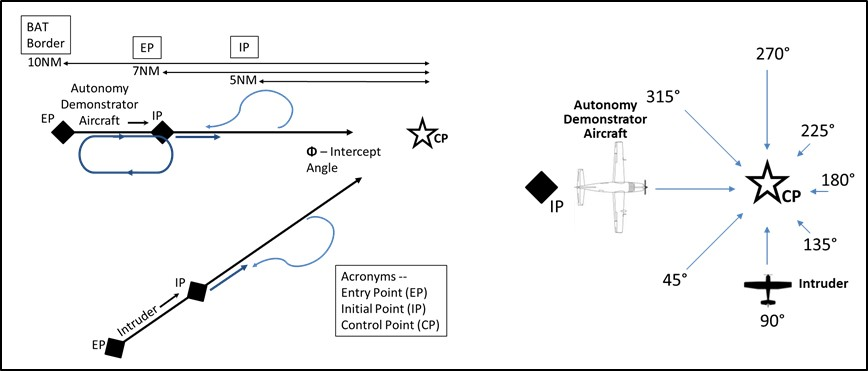
\includegraphics[width=\textwidth]{figures/flight-test.jpg}
	\caption{Flight test plan for evaluation of LEC collision avoidance and RTA safety guarantees}
	\label{fig:flight-test}
\end{figure*}

As described above, two avoidance flight plans were automatically generated on the testbed aircraft, one by the LEC and the other by the backup avoidance planner (which did not use a neural network).
The RTA architecture assessed the two plans and determined which would be flown by the testbed to remain well clear of the intruder.

Flight testing consisted of the live execution of multiple two-aircraft test conditions.  Each test condition specified the following:
\begin{enumerate}
\item A relative heading angle between the testbed aircraft and the intruder
\item The specification to use one of two LECs that were available on the testbed aircraft flight software
\end{enumerate}

Multiple relative heading angles were flown, including a head-on encounter (relative heading = 180 degrees), and other relative headings in 45 degree intervals.
The available LECs were termed the ``good LEC'' and the ``bad LEC.''  The ``good LEC'' was expected to generate safe remain-well-clear trajectories, while the ``bad LEC'' was designed to generate unsafe trajectories, simulating an LEC producing unintended (and unsafe) behaviors.  

During the numerous test conditions flown we made the following general observations:
\begin{itemize}
\item In test conditions where the good LEC was used, the generated avoidance flight plans resulted in safe and standards conformant remain-well-clear avoidance of the intruder.  The RTA functionality successfully assessed the LEC plans as safe, which resulted in the testbed aircraft flying the LEC route.  
\item In test conditions where the bad LEC was used, the generated avoidance flight plans resulted in violation of the remain-well-clear avoidance criteria relative to the intruder.  The RTA functionality successfully assessed the LEC plans as unsafe, which resulted in the testbed aircraft flying the route from the backup avoidance planner.  
\end{itemize}

%There was a case, though, where the bad LEC actually created a route good enough to be standards conformant, and the Collins RTA functionality did judge that route as safe, which resulted in the testbed aircraft flying the LEC route.

There were two interesting test conditions in which we observed unexpected results.  Recall from Section~\ref{sec:rta} that when both plans are assessed as safe but predicted CPA for either occurs at the limit of the prediction horizon, we prefer the plan whose CPA is actually within the prediction horizon.  This situation occurred spontaneously in one of our test conditions, resulting in the RTA functionality choosing (correctly) the backup plan over the LEC.  

In another test condition we were surprised to observe the RTA functionality choosing to fly the plan generated by the bad LEC.  Upon further analysis, we found that both plans were assessed as safe (though the bad LEC plan was just barely safe) and in this case the plan selector logic correctly chose the LEC plan.  However, during execution of the test scenario the RWC separation criteria was violated.  We discovered that several factors combined to place the intruder aircaft ahead of its predicted position, resulting in separation slightly below the RWC requirement.  This condition was possible in our experiment because of an initial design decision to have each of the planners produce only a single avoidance flight plan at the start of a collision encounter, with no updates for any changes that might occur during test execution.  


%For the conclusion:
%- changes/improvements for future demos (more dynamic)